% Options for packages loaded elsewhere
\PassOptionsToPackage{unicode}{hyperref}
\PassOptionsToPackage{hyphens}{url}
%
\documentclass[
]{article}
\usepackage{lmodern}
\usepackage{amssymb,amsmath}
\usepackage{ifxetex,ifluatex}
\ifnum 0\ifxetex 1\fi\ifluatex 1\fi=0 % if pdftex
  \usepackage[T1]{fontenc}
  \usepackage[utf8]{inputenc}
  \usepackage{textcomp} % provide euro and other symbols
\else % if luatex or xetex
  \usepackage{unicode-math}
  \defaultfontfeatures{Scale=MatchLowercase}
  \defaultfontfeatures[\rmfamily]{Ligatures=TeX,Scale=1}
\fi
% Use upquote if available, for straight quotes in verbatim environments
\IfFileExists{upquote.sty}{\usepackage{upquote}}{}
\IfFileExists{microtype.sty}{% use microtype if available
  \usepackage[]{microtype}
  \UseMicrotypeSet[protrusion]{basicmath} % disable protrusion for tt fonts
}{}
\makeatletter
\@ifundefined{KOMAClassName}{% if non-KOMA class
  \IfFileExists{parskip.sty}{%
    \usepackage{parskip}
  }{% else
    \setlength{\parindent}{0pt}
    \setlength{\parskip}{6pt plus 2pt minus 1pt}}
}{% if KOMA class
  \KOMAoptions{parskip=half}}
\makeatother
\usepackage{xcolor}
\IfFileExists{xurl.sty}{\usepackage{xurl}}{} % add URL line breaks if available
\IfFileExists{bookmark.sty}{\usepackage{bookmark}}{\usepackage{hyperref}}
\hypersetup{
  pdftitle={``Identifying and Analyzing Traits Associated with High Performers},
  pdfauthor={Clara Su, Manuel Maldonado, Robert Pimentel and Thomas Pin},
  hidelinks,
  pdfcreator={LaTeX via pandoc}}
\urlstyle{same} % disable monospaced font for URLs
\usepackage[margin=1in]{geometry}
\usepackage{longtable,booktabs}
% Correct order of tables after \paragraph or \subparagraph
\usepackage{etoolbox}
\makeatletter
\patchcmd\longtable{\par}{\if@noskipsec\mbox{}\fi\par}{}{}
\makeatother
% Allow footnotes in longtable head/foot
\IfFileExists{footnotehyper.sty}{\usepackage{footnotehyper}}{\usepackage{footnote}}
\makesavenoteenv{longtable}
\usepackage{graphicx,grffile}
\makeatletter
\def\maxwidth{\ifdim\Gin@nat@width>\linewidth\linewidth\else\Gin@nat@width\fi}
\def\maxheight{\ifdim\Gin@nat@height>\textheight\textheight\else\Gin@nat@height\fi}
\makeatother
% Scale images if necessary, so that they will not overflow the page
% margins by default, and it is still possible to overwrite the defaults
% using explicit options in \includegraphics[width, height, ...]{}
\setkeys{Gin}{width=\maxwidth,height=\maxheight,keepaspectratio}
% Set default figure placement to htbp
\makeatletter
\def\fps@figure{htbp}
\makeatother
\setlength{\emergencystretch}{3em} % prevent overfull lines
\providecommand{\tightlist}{%
  \setlength{\itemsep}{0pt}\setlength{\parskip}{0pt}}
\setcounter{secnumdepth}{-\maxdimen} % remove section numbering

\title{``Identifying and Analyzing Traits Associated with High Performers}
\author{Clara Su, Manuel Maldonado, Robert Pimentel and Thomas Pin}
\date{05/08/2020}

\begin{document}
\maketitle

\hypertarget{glentel}{%
\subsection{Glentel}\label{glentel}}

\begin{itemize}
\tightlist
\item
  \textbf{Mobile Phone Retailer in Canada}
\item
  Joint venture between Rogers Communications and Bell Canada
  Enterprises
\item
  350 locations spread over three banners
\item
  2,000 employees

  \begin{itemize}
  \tightlist
  \item
    Sales Associate
  \item
    Assistant Manager
  \item
    Sales Manager
  \end{itemize}
\end{itemize}

\begin{center}\rule{0.5\linewidth}{0.5pt}\end{center}

\begin{center}\rule{0.5\linewidth}{0.5pt}\end{center}

\begin{center}\rule{0.5\linewidth}{0.5pt}\end{center}

\hypertarget{data-science-problem}{%
\subsection{Data Science Problem}\label{data-science-problem}}

\textbf{HR wishes to understand what are the traits that are associated
with employees who become high performers?''}

This in order to:

\begin{itemize}
\tightlist
\item
  \textbf{Decrease turnover rate} in new hires.
\item
  \textbf{Optimize work force} in function of performance expectation.
\end{itemize}

\hypertarget{current-solution}{%
\subsubsection{\texorpdfstring{\textbf{Current
Solution}}{Current Solution}}\label{current-solution}}

\begin{itemize}
\tightlist
\item
  No quantitative support for high-performing traits looked for in new
  hires.
\end{itemize}

\hypertarget{data}{%
\subsection{Data}\label{data}}

Two sources of Data:

\begin{itemize}
\tightlist
\item
  \textbf{Unstructured Data}

  \begin{itemize}
  \tightlist
  \item
    400-600 Resumes (2019 onwards)
  \end{itemize}
\item
  \textbf{Structured (Tabular)}

  \begin{itemize}
  \tightlist
  \item
    Employee demographics
  \item
    Sales: phone/line ``Activation'' Data (2018 onwards)
  \item
    Compensation tier based on activations
  \item
    Termination reason
  \item
    Promotions
  \item
    Transfers
  \end{itemize}
\end{itemize}

\hypertarget{data-challenges}{%
\subsection{Data Challenges}\label{data-challenges}}

Style\_1.pdf


\includegraphics{../img/project_proposal/09_resume1.png}

Style\_2.docx


\includegraphics{../img/project_proposal/12_resume_3.png}

\begin{itemize}
\tightlist
\item
  Different file formats (PDF's, doc, docx, rtf, txt)
\item
  Different text formats
\end{itemize}

\hypertarget{data-challenges-1}{%
\subsection{Data Challenges}\label{data-challenges-1}}


\includegraphics{../img/project_proposal/10_resume_blank.png}

- Estimate 5\%-8\%* are blank (based off of a sample size of 150)


\includegraphics[width=4.6875in,height=\textheight]{../img/project_proposal/13_eng_fran.png}

- Resume in both French and English

\hypertarget{data-challenges-2}{%
\subsection{Data Challenges}\label{data-challenges-2}}

\begin{itemize}
\tightlist
\item
  Low sample size, limited primarly by resume data.
\end{itemize}

\hypertarget{target-response-variable}{%
\subsection{Target (Response Variable)}\label{target-response-variable}}

\begin{itemize}
\tightlist
\item
  Performance Level: Binary

  \begin{itemize}
  \tightlist
  \item
    High Performer (1)
  \item
    Low Performer (0)
  \end{itemize}
\end{itemize}

\begin{itemize}
\tightlist
\item
  Requested by the company, based on their payroll tier reached.
\item
  Influenced by sample size.
\end{itemize}

\hypertarget{target-response-variable-1}{%
\subsection{Target (Response
Variable)}\label{target-response-variable-1}}

\begin{itemize}
\tightlist
\item
  Pay achievement level
\end{itemize}

\hypertarget{data-preparation-ideal-data-format}{%
\subsection{Data Preparation: Ideal Data
Format}\label{data-preparation-ideal-data-format}}

\begin{longtable}[]{@{}llrrrl@{}}
\toprule
Employee\_ID & Text & Feature2 & Feature3 & Feature\_n &
Target\tabularnewline
\midrule
\endhead
231 & \ldots{} & 0 & 1 & 0 & High Performer\tabularnewline
456 & \ldots{} & 1 & 1 & 1 & Non-High Performer\tabularnewline
790 & \ldots{} & 0 & 0 & 1 & Non-High Performer\tabularnewline
\bottomrule
\end{longtable}

\hypertarget{potential-features}{%
\subsection{Potential Features}\label{potential-features}}

\begin{itemize}
\tightlist
\item
  \textbf{Hire Type}

  \begin{itemize}
  \tightlist
  \item
    Re-hire
  \item
    Referral
  \end{itemize}
\end{itemize}

\begin{itemize}
\tightlist
\item
  \textbf{Resume Features}

  \begin{itemize}
  \tightlist
  \item
    Education
  \item
    Experience
  \item
    Job hopping
  \item
    Job experience (type and time)
  \item
    Spelling mistakes
  \item
    Language
  \end{itemize}
\end{itemize}

\hypertarget{natural-language-processing-nlp}{%
\subsection{Natural Language Processing
(NLP)}\label{natural-language-processing-nlp}}

\begin{itemize}
\tightlist
\item
  Extracting corpus from resumes
\item
  Pre-processing (stopwords, special characters, punctuation)
\end{itemize}

\begin{itemize}
\tightlist
\item
  count vectorizer (BOW):

  \begin{itemize}
  \tightlist
  \item
    We expect to identify keywords associated to high performance
  \end{itemize}
\end{itemize}

\begin{itemize}
\tightlist
\item
  Topic modelling:

  \begin{itemize}
  \tightlist
  \item
    Additional insight for feature engineering
  \end{itemize}
\end{itemize}

\hypertarget{feature-engineering}{%
\subsection{Feature Engineering}\label{feature-engineering}}

\begin{longtable}[]{@{}lrrrrrl@{}}
\toprule
Resume & College & Retail & Teamwork & Sales & Communication &
Target\tabularnewline
\midrule
\endhead
Resume 1 & 1 & 0 & 1 & 0 & 1 & High Performer (1)\tabularnewline
Resume 2 & 0 & 1 & 1 & 0 & 1 & Non-High Performer (0)\tabularnewline
\bottomrule
\end{longtable}

\begin{itemize}
\tightlist
\item
  We expect to mix count vectorizer features and engineered features.
\end{itemize}

\hypertarget{machine-learning-pipeline}{%
\subsection{Machine Learning Pipeline}\label{machine-learning-pipeline}}

\begin{enumerate}
\def\labelenumi{\arabic{enumi}.}
\tightlist
\item
  Feature Scaling
\item
  Cross validation
\item
  Hyperparameter optimization
\item
  Feature Selection (RFE)
\item
  Model training
\item
  Model Interpretation
\end{enumerate}

\textbf{Models}

\begin{itemize}
\tightlist
\item
  Baseline : logistic regression
\item
  Additional classifiers:

  \begin{itemize}
  \tightlist
  \item
    SVM
  \item
    Random Forest
  \item
    Multilayer perceptron
  \end{itemize}
\end{itemize}

\hypertarget{complex-model-limitations}{%
\subsection{Complex Model Limitations}\label{complex-model-limitations}}

\textbf{LSTMs}

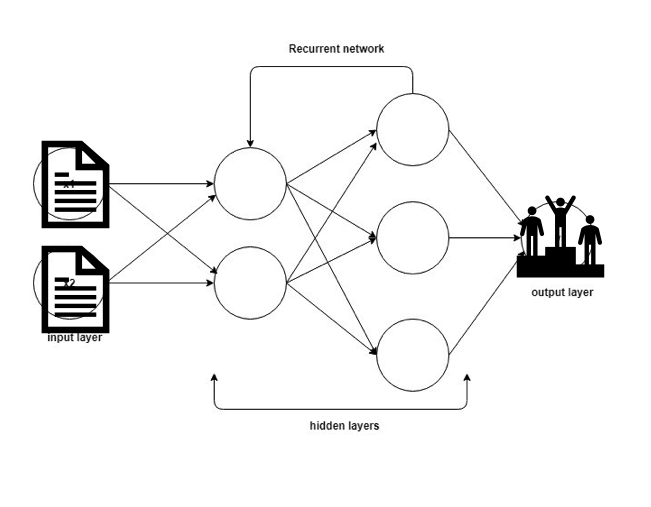
\includegraphics[width=4.6875in,height=\textheight]{../img/project_proposal/08_LSTM.png}

\begin{itemize}
\tightlist
\item
  Low sample size (overall aprox 400 observations)
\item
  Deep learning models are hard to interpret.
\end{itemize}

\hypertarget{plan}{%
\subsection{Plan}\label{plan}}

\textbf{Week 1} May 4 - May 8

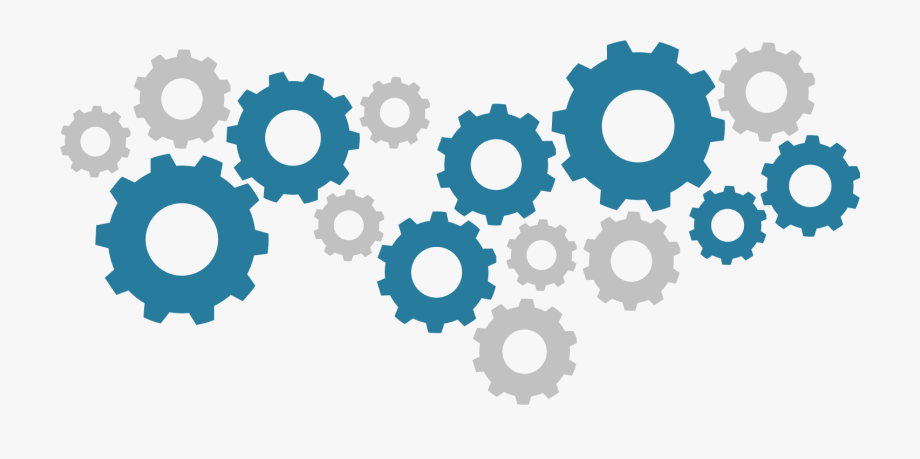
\includegraphics[width=2.60417in,height=\textheight]{../img/project_proposal/28_process.png}

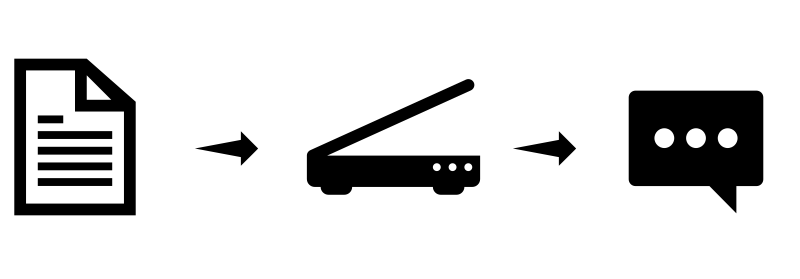
\includegraphics[width=4.6875in,height=\textheight]{../img/project_proposal/15_week1.png}

\begin{itemize}
\tightlist
\item
  Understanding/defining problem to be solved with Glentel
\item
  Methodology research and definition
\item
  Preliminary EDA on Tabular Datasets
\end{itemize}

\begin{itemize}
\tightlist
\item
  Company still extracting resume information.
\end{itemize}

\hypertarget{plan-1}{%
\subsection{Plan}\label{plan-1}}

\textbf{Week 2} May 11 - May 15

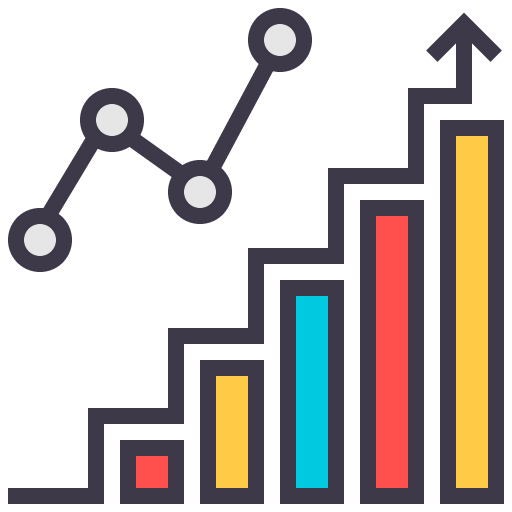
\includegraphics[width=1.5625in,height=\textheight]{../img/project_proposal/17_eda.png}

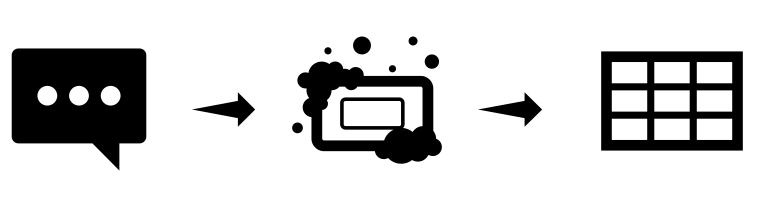
\includegraphics[width=4.94792in,height=\textheight]{../img/project_proposal/16_week2.png}

\begin{itemize}
\tightlist
\item
  Final Proposal to partners
\item
  EDA
\end{itemize}

\begin{itemize}
\tightlist
\item
  Resume - Loading and Processing :

  \begin{itemize}
  \tightlist
  \item
    Special characters
  \item
    Stop words
  \item
    Lemmatization
  \end{itemize}
\end{itemize}

\hypertarget{plan-2}{%
\subsection{Plan}\label{plan-2}}

\textbf{Week 3-4} May 18 - May 29

\textbf{NLP}

\begin{itemize}
\item
  Count Vectorizer
\item
  Topic Modelling
\item
  Feature Engineering

  \begin{itemize}
  \tightlist
  \item
    Based on insights of the previous
  \item
    Based on partner's expertise
  \item
    Based on data scientist's criteria.
  \end{itemize}
\end{itemize}

\hypertarget{plan-3}{%
\subsection{Plan}\label{plan-3}}

\textbf{Week 5} Jun 1 - Jun 5

\textbf{Baseline Model Creation: Logistic Regression}

\begin{itemize}
\tightlist
\item
  Machine Learning Pipeline

  \begin{itemize}
  \tightlist
  \item
    scaling
  \item
    cross validation
  \item
    hyperparameter
  \item
    Feature Selection
  \item
    Measuring model Performance
  \end{itemize}
\end{itemize}

\hypertarget{plan-4}{%
\subsection{Plan}\label{plan-4}}

\textbf{Week 6-7} Jun 8 - Jun 12

\textbf{Challenging the baseline model with additional classifiers}

\begin{itemize}
\tightlist
\item
  Random Forest
\item
  SVM
\item
  Multilayer perceptron
\end{itemize}

\hypertarget{plan-5}{%
\subsection{Plan}\label{plan-5}}

\textbf{Week 8} Jun 15 - Jun 19

\begin{itemize}
\tightlist
\item
  Result documentation and comparison
\item
  Final Model Selection
\item
  Presentation preparation
\end{itemize}

\hypertarget{gantt-chart}{%
\subsection{Gantt Chart}\label{gantt-chart}}

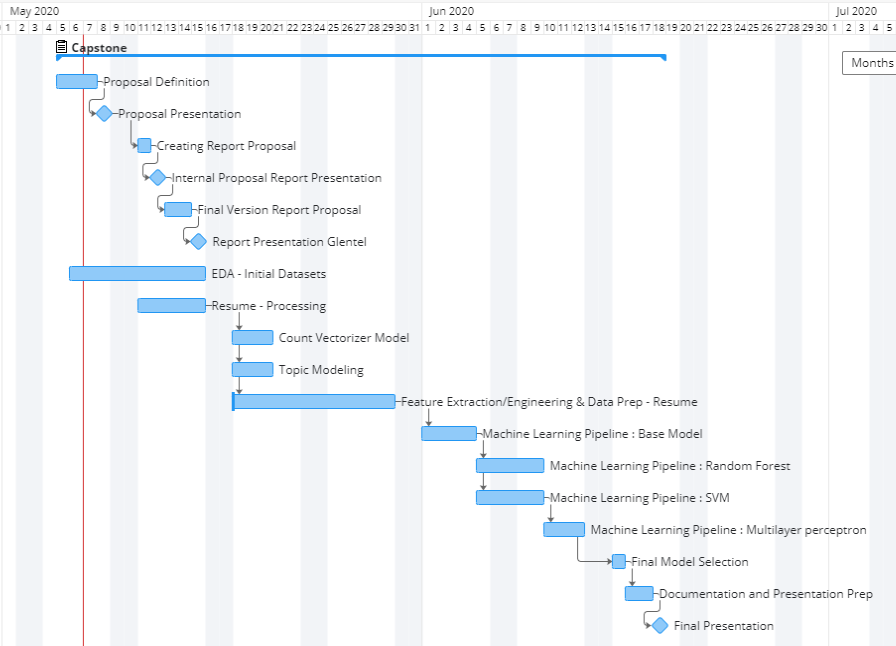
\includegraphics[width=7.29167in,height=\textheight]{../img/project_proposal/22_gantt_chart.png}

\hypertarget{questions}{%
\subsection{Questions?}\label{questions}}

\end{document}
